\documentclass[11pt,compress,t,notes=noshow, aspectratio=169, xcolor=table,dvipsnames]{beamer}

\usepackage{../../style/lmu-lecture}

% %  New colors
\definecolor{ggRed}{HTML}{F8766D}
\definecolor{ggGreen}{HTML}{00BFC4}
\definecolor{rep}{HTML}{3646f1}
\definecolor{cice}{HTML}{00BFFF}
\definecolor{mygreen}{HTML}{0FA90F}
\definecolor{amber}{rgb}{0.9, 0.7, 0.1}

\newcommand{\highlightICE}[1]{\colorbox{cice}{$\displaystyle #1$}}
\newcommand{\highlight}[1]{\colorbox{orange}{$\displaystyle #1$}}
\newcommand{\highlightYG}[1]{\colorbox{YellowGreen!50}{$\displaystyle #1$}}
\newcommand{\highlightFG}[1]{\colorbox{ForestGreen!70}{$\displaystyle #1$}}

\usepackage{tikz}
\usetikzlibrary{shapes,arrows,automata,positioning,calc,chains,trees, shadows}
\tikzset{
  %Define standard arrow tip
  >=stealth',
  %Define style for boxes
  punkt/.style={
    rectangle,
    rounded corners,
    draw=black, very thick,
    text width=6.5em,
    minimum height=2em,
    text centered},
  % Define arrow style
  pil/.style={
    ->,
    thick,
    shorten <=2pt,
    shorten >=2pt,}
}

% definition of the style
\tikzset{exampleblock/.style={rounded corners,rectangle split, rectangle split parts=4, draw, 
rectangle split part fill={gray!20, gray!20, cice!20, orange!20},minimum width=0.3\textwidth
}}
\tikzset{main node/.style={rectangle,draw,minimum size=1cm,inner sep=4pt},}
\usetikzlibrary{calc}
\usetikzlibrary{chains, positioning, arrows, trees, shadows}
%\input{figure/gear.tex}
%http://tex.stackexchange.com/questions/6135/how-to-make-beamer-overlays-with-tikz-node
\tikzset{
  %Style of the black box
  bbox/.style={draw, fill=black, minimum size=3cm,
  label={[white, yshift=-1.3em]above:$in$},
  label={[white, yshift=1.3em]below:$out$},
  label={[rotate = 90, xshift=1em, yshift=0.5em]left:Black-Box}
  },
  multiple/.style={double copy shadow={shadow xshift=1.5ex,shadow
  yshift=-0.5ex,draw=black!30,fill=white}},
}

% for overlay box
\usetikzlibrary{backgrounds,shapes.multipart}
\pgfdeclarelayer{myback}
\pgfsetlayers{background,main,myback} %<= insert the myback 
% after the "main" to display the content in front of the usual content


% Defines macros and environments
% This file is included in slides and exercises

% Rarely used fontstyle for R packages, used only in 
% - forests/slides-forests-benchmark.tex
% - exercises/single-exercises/methods_l_1.Rnw
% - slides/cart/attic/slides_extra_trees.Rnw
\newcommand{\pkg}[1]{{\fontseries{b}\selectfont #1}}

% Spacing helpers, used often (mostly in exercises for \dlz)
\newcommand{\lz}{\vspace{0.5cm}} % vertical space (used often in slides)
\newcommand{\dlz}{\vspace{1cm}}  % double vertical space (used often in exercises, never in slides)
\newcommand{\oneliner}[1] % Oneliner for important statements, used e.g. in iml, algods
{\begin{block}{}\begin{center}\begin{Large}#1\end{Large}\end{center}\end{block}}

% Don't know if this is used or needed, remove?
% textcolor that works in mathmode
% https://tex.stackexchange.com/a/261480
% Used e.g. in forests/slides-forests-bagging.tex
% [...] \textcolor{blue}{\tfrac{1}{M}\sum^M_{m} [...]
% \makeatletter
% \renewcommand*{\@textcolor}[3]{%
%   \protect\leavevmode
%   \begingroup
%     \color#1{#2}#3%
%   \endgroup
% }
% \makeatother


\title{Interpretable Machine Learning}
% \author{LMU}
%\institute{\href{https://compstat-lmu.github.io/lecture_iml/}{compstat-lmu.github.io/lecture\_iml}}
\date{}



\begin{document}

\newcommand{\titlefigure}{figure/sim1_dt_split1.png}
\newcommand{\learninggoals}{
\item Interaction quantification
\item REPID interaction importance
}

\lecturechapter{Regional Effects}
\lecture{Interpretable Machine Learning}



\begin{frame}{Interaction quantification}
It's helpful to know not just how another feature changes the marginal effect of $x_S$ but how strong that interaction is and want to rank features by it.

\textbf{Approaches:}
\begin{itemize}
    \item \textbf{H-Statistics:} Variance of the deviation between the joint PDP and the sum of marginal PDPs (larger variance $\Rightarrow$ stronger interaction).
    \item \textbf{Greenwell’s Interaction Index:} Difference between the variance of the PDP and the mean variance of centered ICE curves for the same feature pair.
    \item \textbf{SHAP interaction index (\citebutton{Herbinger et al. (2022)}{https://proceedings.mlr.press/v151/herbinger22a.html}, \citebutton{Lundberg et al. 2018}{https://doi.org/10.48550/arXiv.1802.03888}):} Proportion of all two-way interactions with $x_i$  to which the $j$-th feature contributes.
\end{itemize}

\pause

\textbf{Pitfalls:}
\begin{itemize}
    \item The values of H-Statistic and the Greenwell’s Interaction Index are influenced by the
 main effects of the two regarded features.
    \item SHAP interaction index does not suffer from main effect problem. However, correlation between the two features can bias the interaction value. Same applies to the H-Statistic.  
\end{itemize}

\end{frame}

\begin{frame}{REPID Interaction Importance}

\begin{columns}[T, totalwidth=\textwidth]
    \begin{column}{0.60\textwidth}

\textbf{On parent node level (for {\color{mygreen}$\mathcal{N}_{parent}$}):}
%Relative interaction importance for each parent node :
$$
   intImp({\color{mygreen}{\mathcal{N}_{parent}}}) = \frac{\mathcal{R}({\color{mygreen}\mathcal{N}_{parent}}) - (\mathcal{R}({\color{amber}\mathcal{N}_{left}}) + \mathcal{R}({\color{red}\mathcal{N}_{right}}))}{\mathcal{R}({\color{blue}\mathcal{N}})} 
$$
\textbf{Interpretation:}
Reduction of ICE curve variance after one split of $\mathcal{N}_{parent}$ into $\mathcal{N}_{left}$ and $\mathcal{N}_{right}$ 
relative to the ICE curve variance in the root node $\mathcal{N}$.

\medskip

\begin{center}
      \resizebox{0.5\linewidth}{!}{
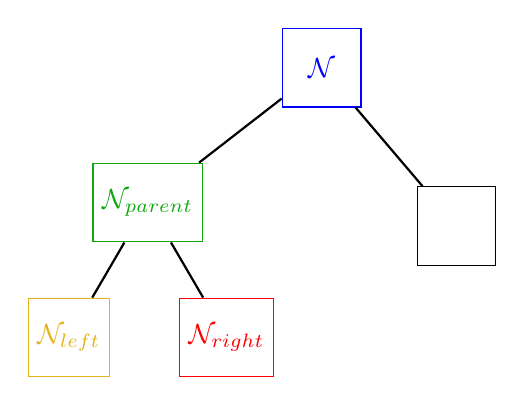
\begin{tikzpicture}
    \usetikzlibrary{arrows}
    \usetikzlibrary{shapes}

    % Define node styles
    \tikzset{
        treenode/.style={draw, rectangle, minimum size=1cm, text centered},
        N/.style={draw, rectangle, minimum size=1cm, text centered, color=blue, text=blue},
        Np/.style={draw, rectangle, minimum size=1cm, text centered, color=mygreen, text=mygreen},
        Nl/.style={draw, rectangle, minimum size=1cm, text centered, color=amber, text=amber},
        Nr/.style={draw, rectangle, minimum size=1cm, text centered, color=red, text=red}
    }

    % Nodes
    \node [N] (a0) {$\mathcal{N}$}; % Top node
    \node [treenode, below right=1cm and 0.7cm of a0] (a1) {}; % Bottom right node
    \node [Np, below left=0.7cm and 1cm of a0] (a2) {$\mathcal{N}_{parent}$}; % Bottom center node
    \node [Nl, below=0.7cm of a2, xshift=-1cm] (a3) {$\mathcal{N}_{left}$}; % Bottom left node
    \node [Nr, below=0.7cm of a2, xshift=1cm] (a4) {$\mathcal{N}_{right}$}; % Bottom right node from center

    % Lines
    \draw [thick] (a0) -- (a1);
    \draw [thick] (a0) -- (a2);
    \draw [thick] (a2) -- (a3);
    \draw [thick] (a2) -- (a4);
\end{tikzpicture}}

\end{center}
    \end{column}
\pause
    \begin{column}{0.4\textwidth}
  %\centering\includegraphics[width = 0.6\textwidth]{figure/tree_expl.png}
 \centering
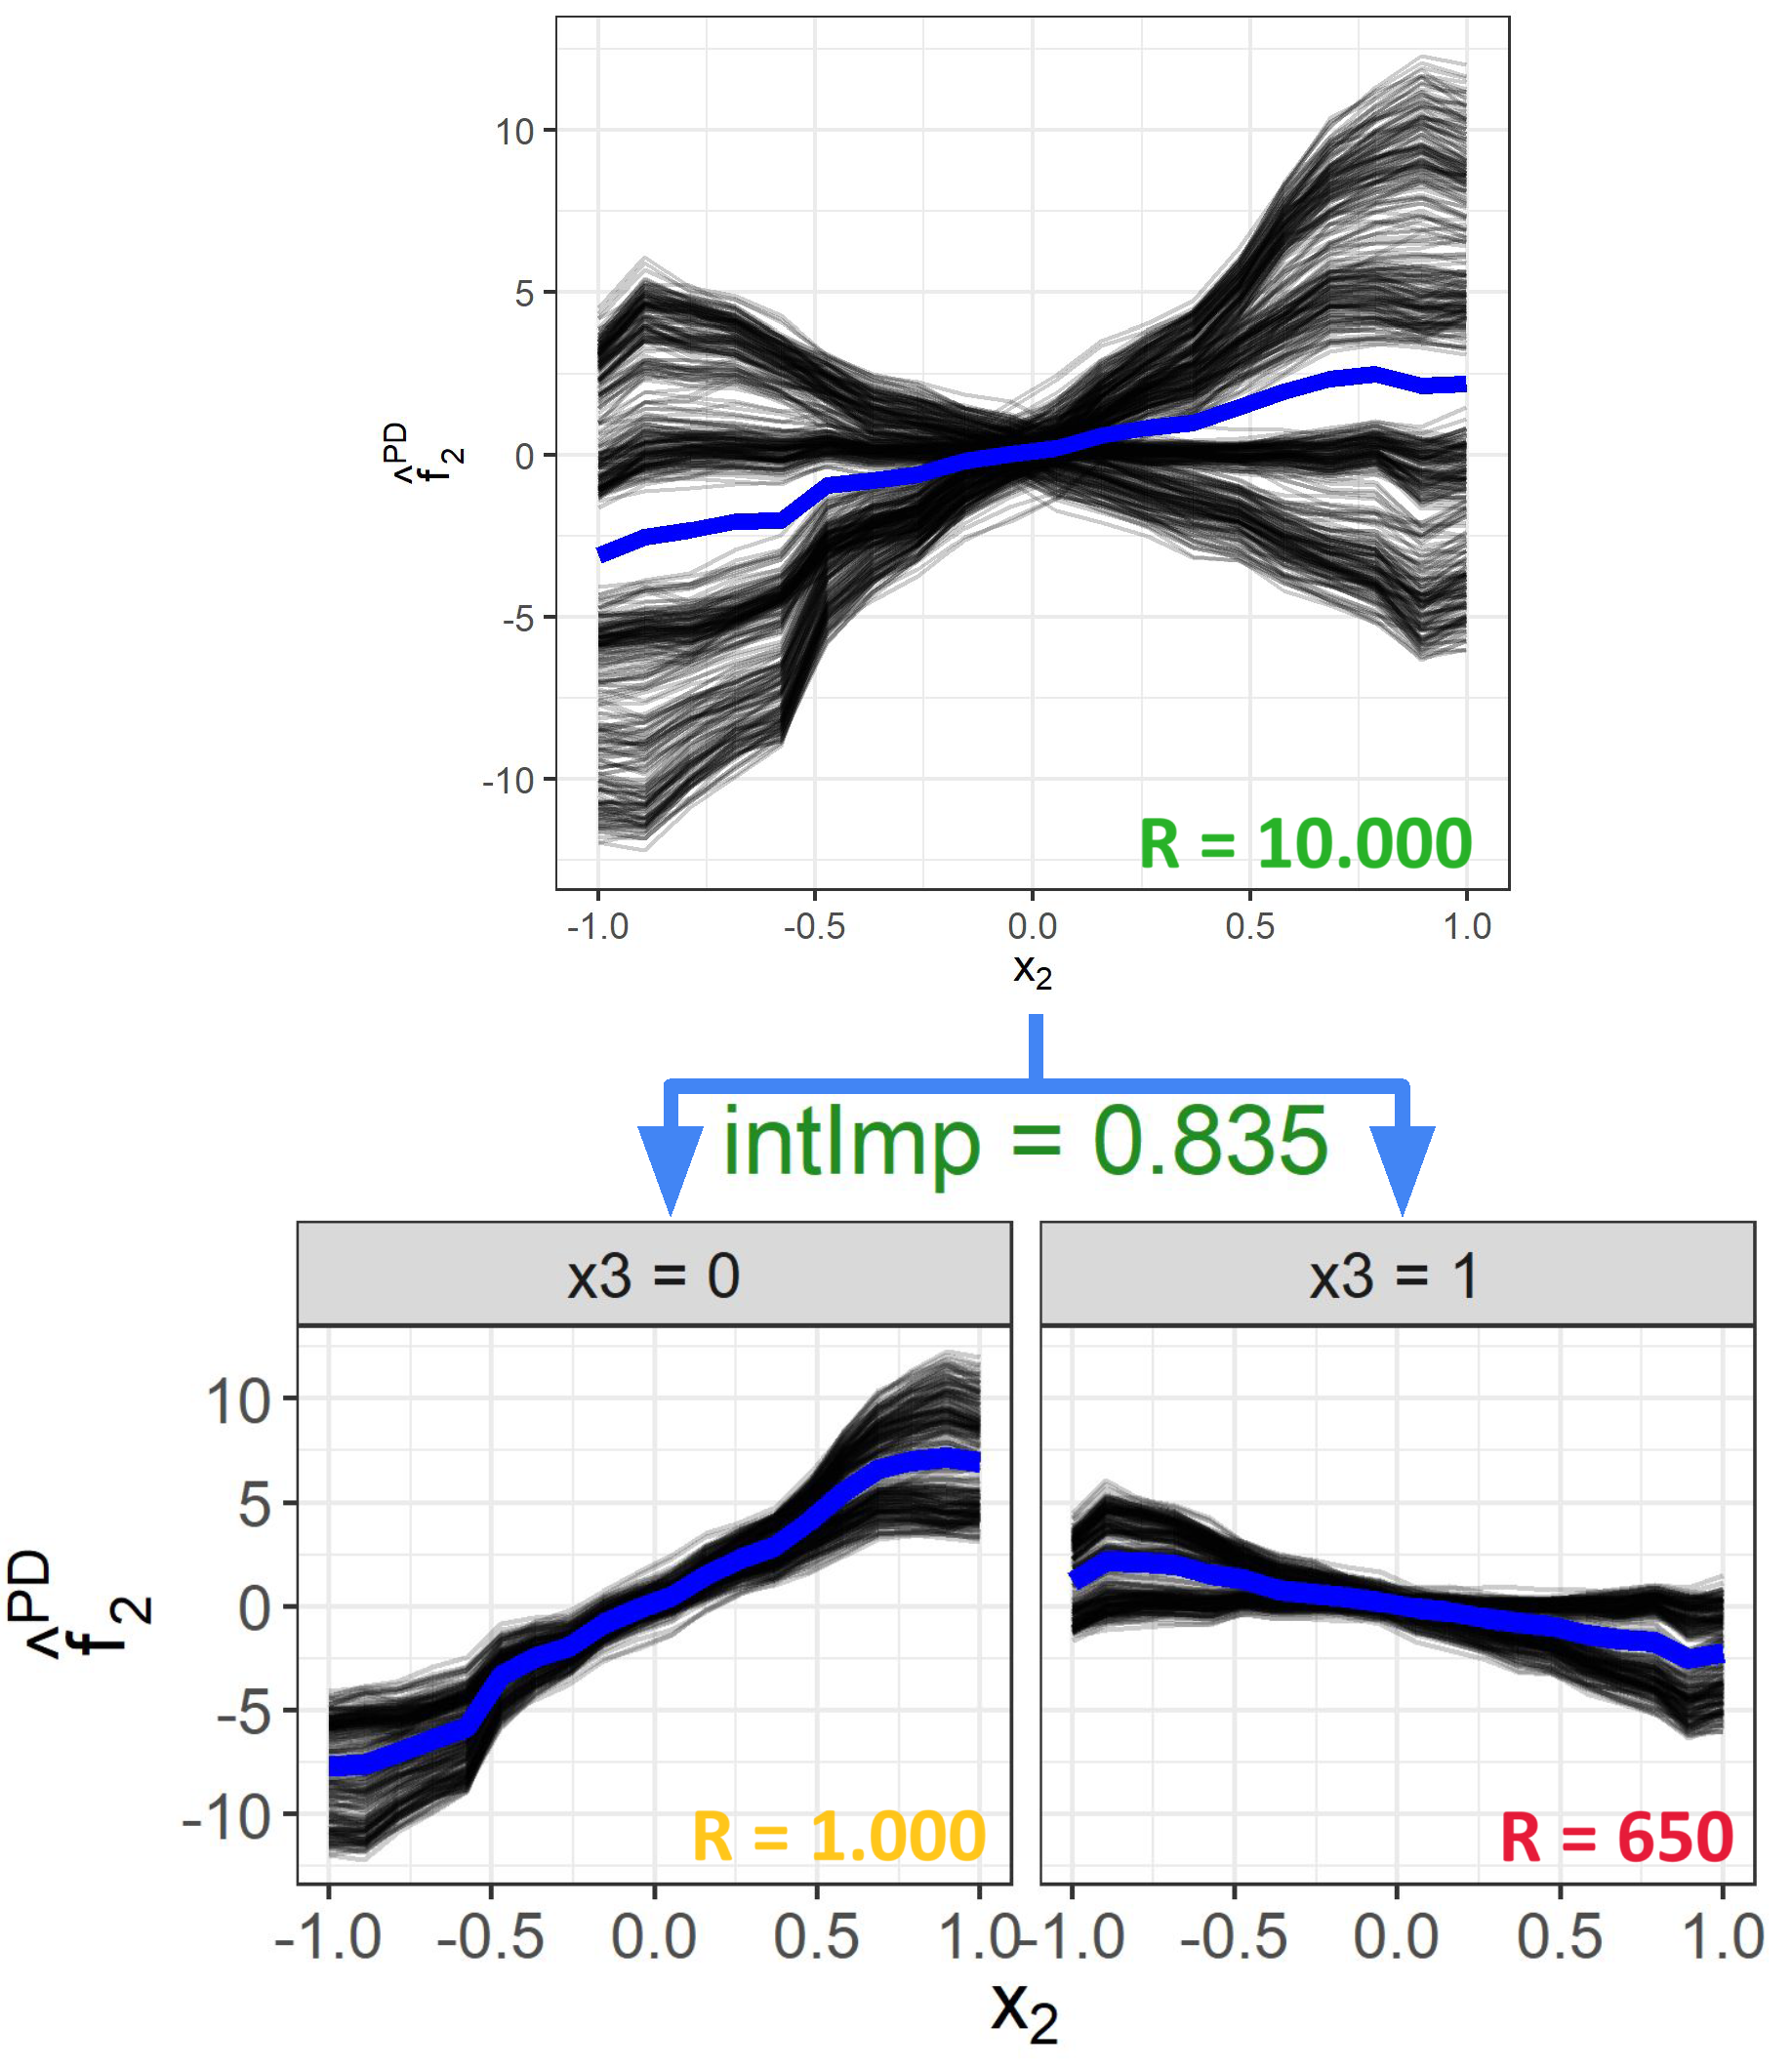
\includegraphics[width = 0.95\textwidth]{figure/sim1_fake.png}

Split reduces 83.5\% of variance.
    \end{column}
\end{columns}

\end{frame}


\begin{frame}{REPID Interaction Importance}
    
\begin{columns}[T, totalwidth=\textwidth]%, totalwidth=\textwidth]
    \begin{column}{0.5\textwidth}

\textbf{On feature level (for $x_j$):} 
%Relative interaction importance for feature $x_j$:
%We denote this subset by $\mathcal{B}_j \subset \mathcal{B}_P$ and the relative interaction importance by
\medskip

\centerline{$\textstyle
   intImp_j = \sum\nolimits_{i \in \mathcal{B}_j} intImp(\mathcal{N}_i)$}

\medskip

%\textbf{$\bm{intImp(\mathcal{N}_P)}$: risk reduction after one split relative to the root node risk}
%where $\mathcal{B}_j$ indexes parent nodes where splits are based on $x_j$.
where $\mathcal{B}_j$ indexes parent nodes split by $x_j$.

\medskip

\textbf{Interpretation:}
Overall reduction of ICE curve variance due to splits by $X_j$ (in \%).

\medskip

\textbf{Example:} For $X_1 \Rightarrow$  {\color{orange} $\mathcal{B}_1 = \{0, 2, 3\}$}
    \begin{center}
      \resizebox{1\textwidth}{!}{
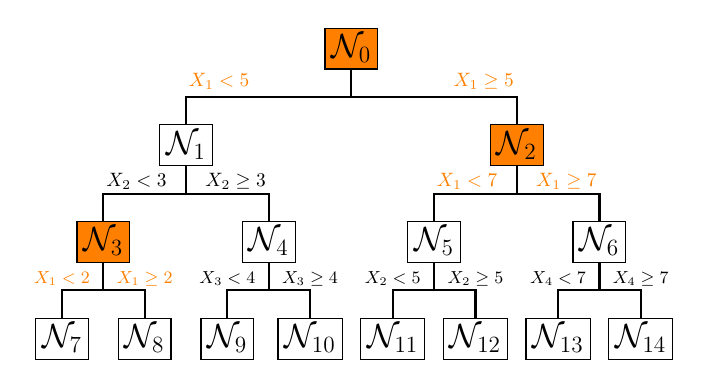
\begin{tikzpicture}[scale=0.7, transform shape]
    \tikzset{treenode/.style={draw, rectangle, font=\LARGE}}
    \tikzset{line/.style={draw, thick}}

    % Root node
    \node [treenode, fill=orange] (a0) {$\mathcal{N}_0$};

    % Level 1 nodes
    \node [treenode, below=1cm of a0, xshift=-3cm] (a1) {$\mathcal{N}_1$};
    \node [treenode, fill=orange, below=1cm of a0, xshift=3cm] (a2) {$\mathcal{N}_2$};

    % Level 2 nodes
    \node [treenode, fill=orange, below=1cm of a1, xshift=-1.5cm] (a3) {$\mathcal{N}_3$};
    \node [treenode, below=1cm of a1, xshift=1.5cm] (a4) {$\mathcal{N}_4$};
    \node [treenode, below=1cm of a2, xshift=-1.5cm] (a5) {$\mathcal{N}_5$};
    \node [treenode, below=1cm of a2, xshift=1.5cm] (a6) {$\mathcal{N}_6$};

    % Level 3 nodes
    \node [treenode, below=1cm of a3, xshift=-0.75cm] (a7) {$\mathcal{N}_7$};
    \node [treenode, below=1cm of a3, xshift=0.75cm] (a8) {$\mathcal{N}_8$};
    \node [treenode, below=1cm of a4, xshift=-0.75cm] (a9) {$\mathcal{N}_9$};
    \node [treenode, below=1cm of a4, xshift=0.75cm] (a10) {$\mathcal{N}_{10}$};
    \node [treenode, below=1cm of a5, xshift=-0.75cm] (a11) {$\mathcal{N}_{11}$};
    \node [treenode, below=1cm of a5, xshift=0.75cm] (a12) {$\mathcal{N}_{12}$};
    \node [treenode, below=1cm of a6, xshift=-0.75cm] (a13) {$\mathcal{N}_{13}$};
    \node [treenode, below=1cm of a6, xshift=0.75cm] (a14) {$\mathcal{N}_{14}$};

    % Edges and labels
    \path [line] (a0.south) -- + (0,-0.5cm) -| (a1.north) node [pos=0.4, above, color=orange] {$X_1 < 5$};
    \path [line] (a0.south) -- + (0,-0.5cm) -| (a2.north) node [pos=0.4, above, color=orange] {$X_1 \geq 5$};

    \path [line] (a1.south) -- + (0,-0.5cm) -| (a3.north) node [pos=0.3, above, yshift = -0.05cm] {$X_2 < 3$};
    \path [line] (a1.south) -- + (0,-0.5cm) -| (a4.north) node [pos=0.3, above, yshift = -0.05cm] {$X_2 \geq 3$};

    \path [line] (a2.south) -- + (0,-0.5cm) -| (a5.north) node [pos=0.3, above, color=orange, yshift = -0.05cm] {$X_1 < 7$};
    \path [line] (a2.south) -- + (0,-0.5cm) -| (a6.north) node [pos=0.3, above, color=orange, yshift = -0.05cm] {$X_1 \geq 7$};

    \path [line] (a3.south) -- + (0,-0.5cm) -| (a7.north) node [pos=0.5, above, color=orange, yshift = -0.05cm] {\small $X_1 < 2$};
    \path [line] (a3.south) -- + (0,-0.5cm) -| (a8.north) node [pos=0.5, above, color=orange, yshift = -0.05cm] {\small $X_1 \geq 2$};

    \path [line] (a4.south) -- + (0,-0.5cm) -| (a9.north) node [pos=0.5, above, yshift = -0.05cm] {\small $X_3 < 4$};
    \path [line] (a4.south) -- + (0,-0.5cm) -| (a10.north) node [pos=0.5, above, yshift = -0.05cm] {\small $X_3 \geq 4$};

    \path [line] (a5.south) -- + (0,-0.5cm) -| (a11.north) node [pos=0.5, above, yshift = -0.05cm] {\small $X_2 < 5$};
    \path [line] (a5.south) -- + (0,-0.5cm) -| (a12.north) node [pos=0.5, above, yshift = -0.05cm] {\small $X_2 \geq 5$};

    \path [line] (a6.south) -- + (0,-0.5cm) -| (a13.north) node [pos=0.5, above, yshift = -0.05cm] {\small $X_4 < 7$};
    \path [line] (a6.south) -- + (0,-0.5cm) -| (a14.north) node [pos=0.5, above, yshift = -0.05cm] {\small $X_4 \geq 7$};

\end{tikzpicture}}
    \end{center}
    \end{column}
\pause
    \begin{column}{0.52\textwidth}


    \centering
    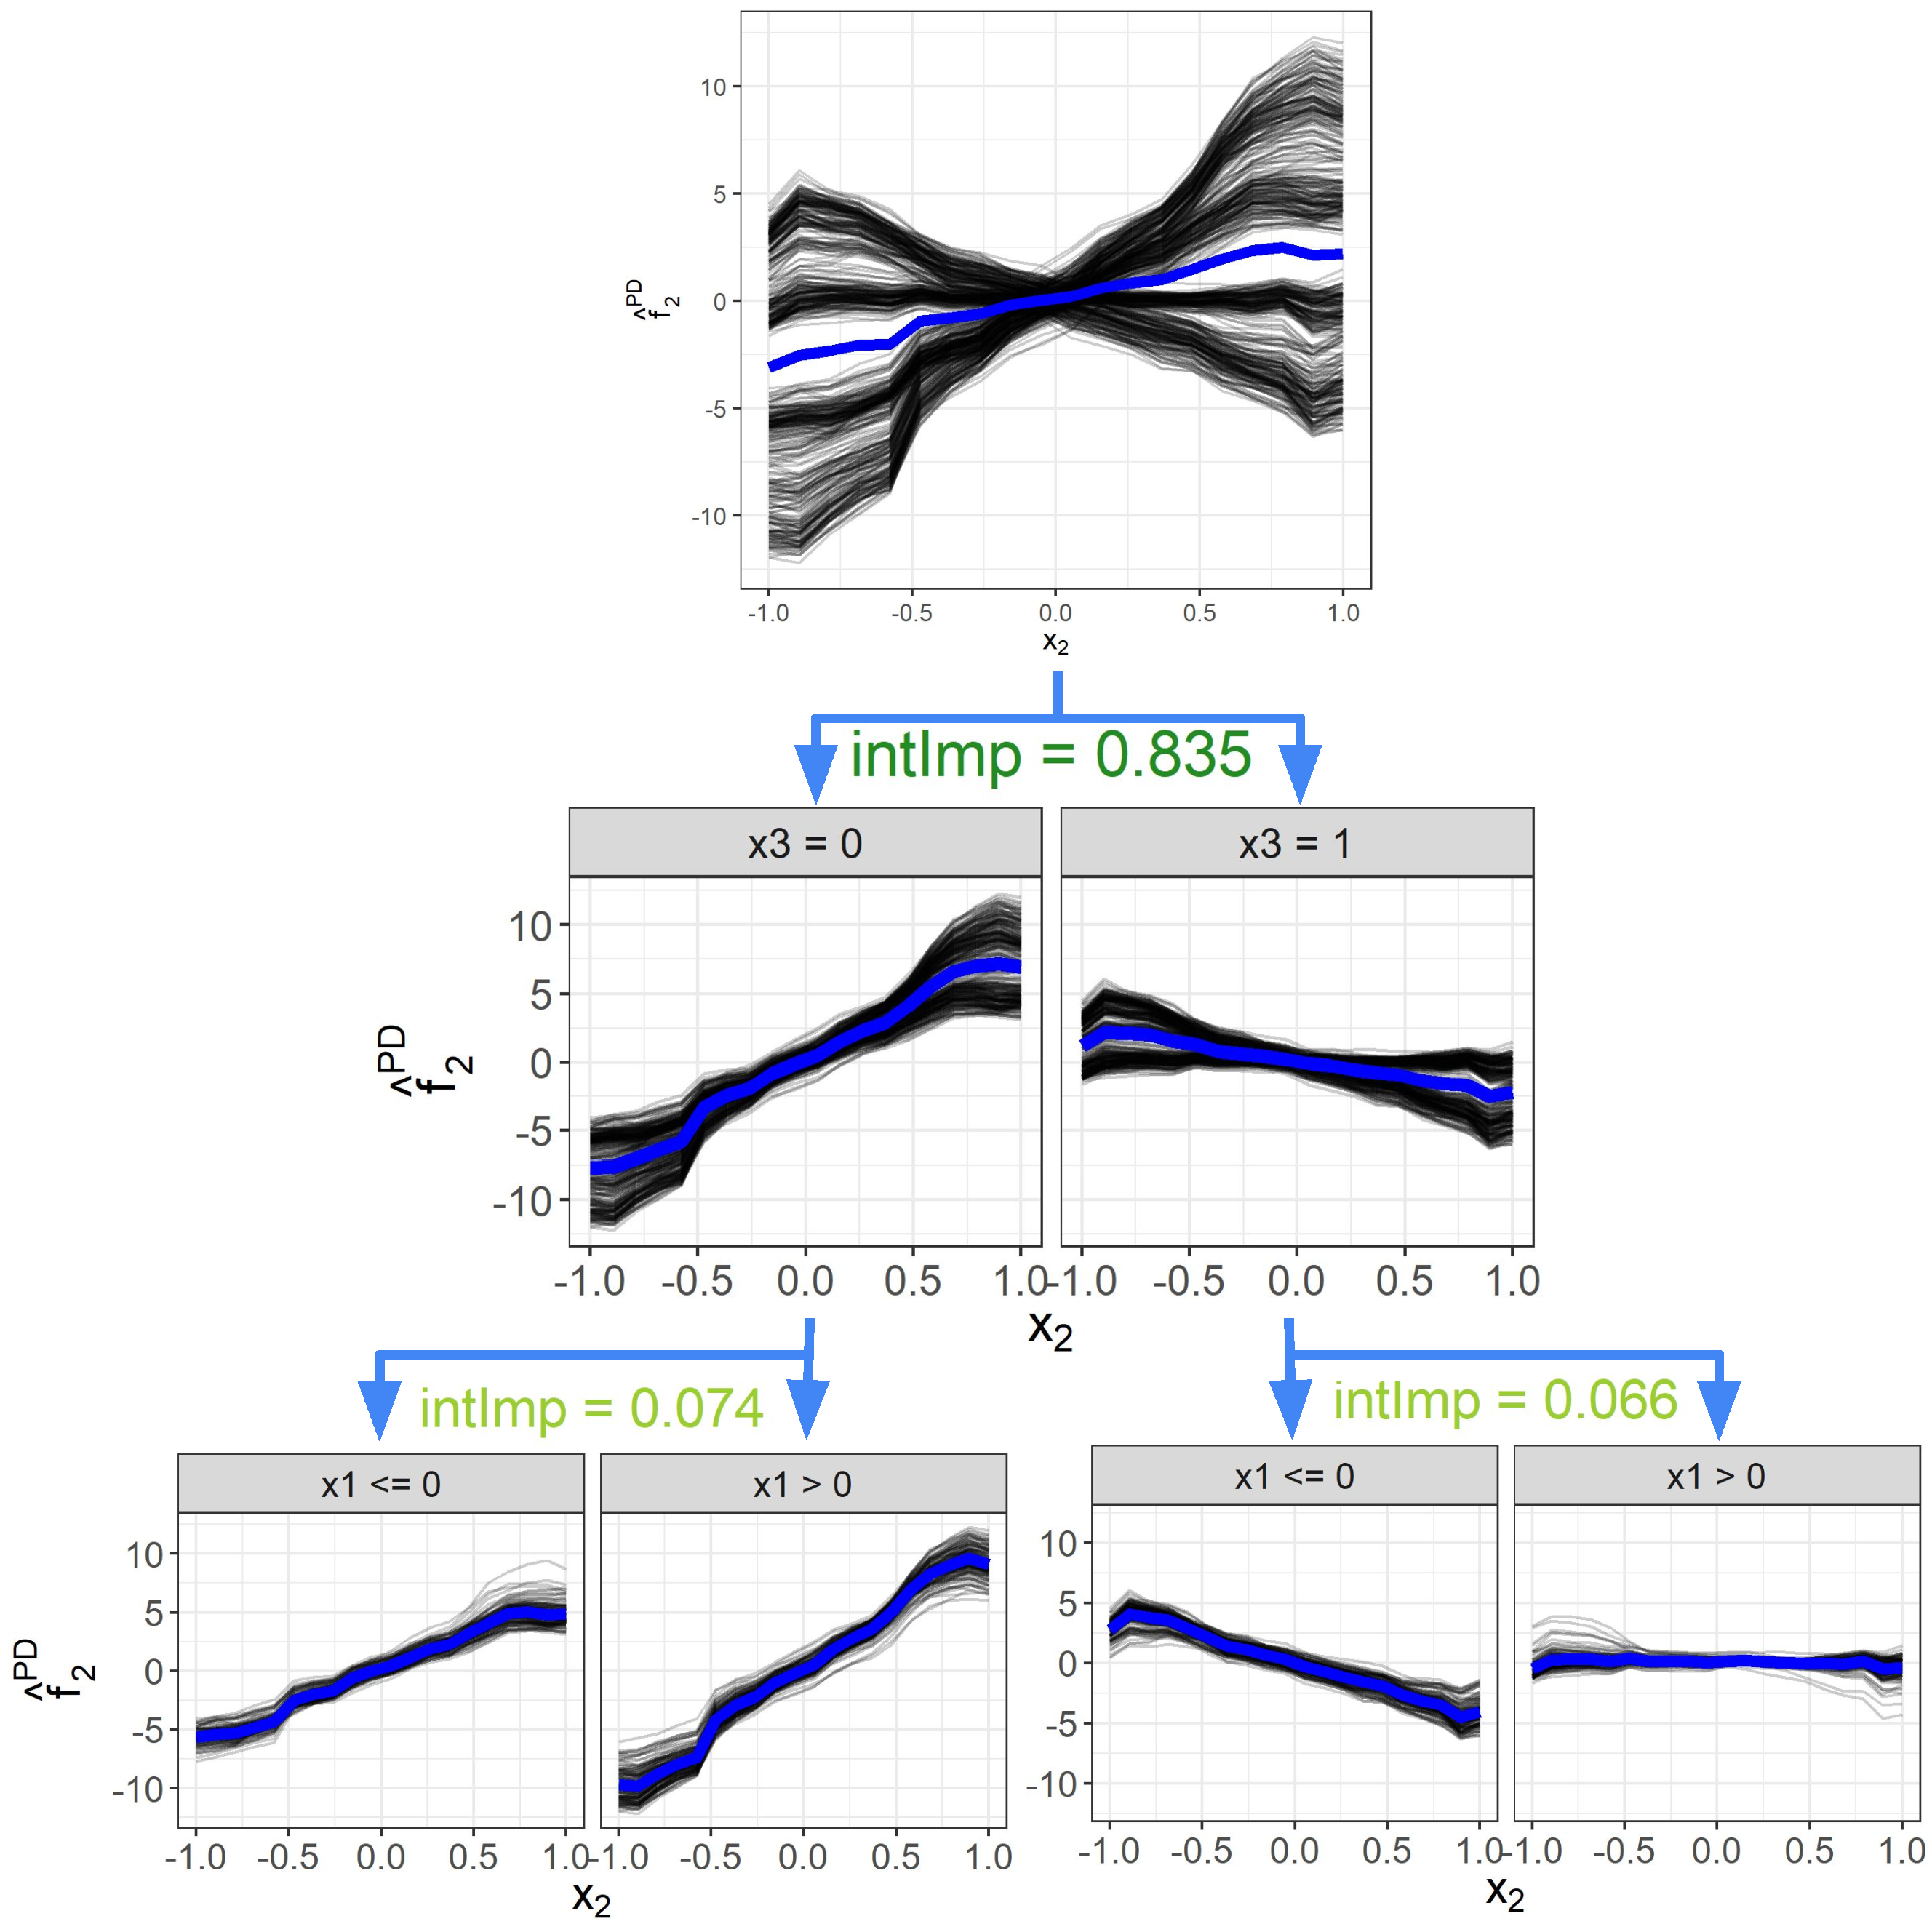
\includegraphics[width=\textwidth]{figure/sim1}
    
    \textbf{Note:} \textit{intImp} can also be used as a stopping criterion.
     %\begin{minipage}[t]{.5\textwidth}
    %   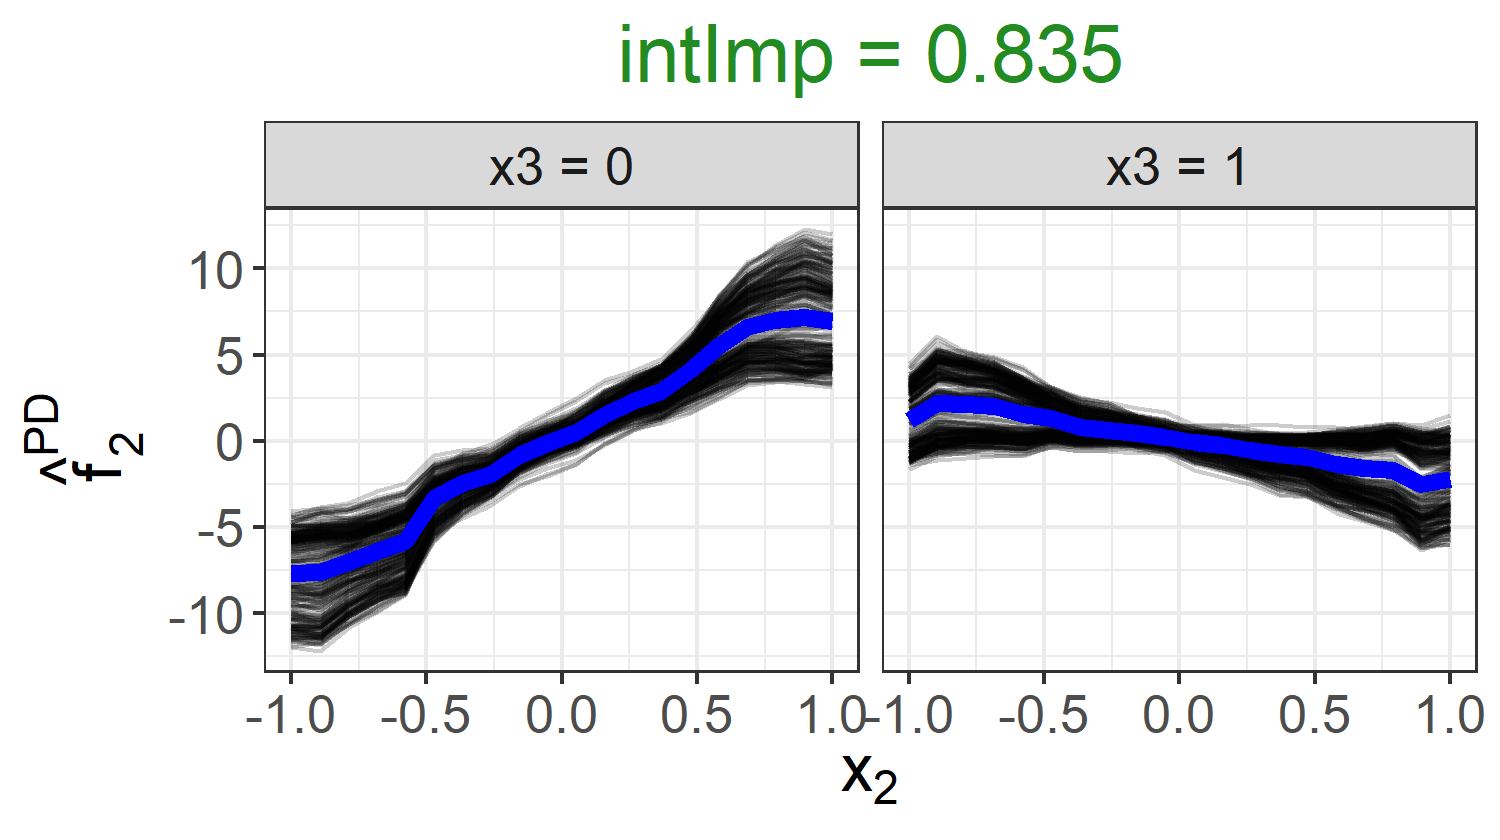
\includegraphics[width=0.37\textwidth]{figure/sim1_dt_split1.png}
    %   \scalebox{1}{
    %   \hspace{15pt} 
    %   \begin{tikzpicture}
    %   \usetikzlibrary{arrows}
    %     \usetikzlibrary{shapes}
    %      \tikzset{treenode/.style={draw}}
    %      \tikzset{line/.style={draw, thick}}
    %     \node [treenode](a0) {} ; [below=1pt,at=(4,0)]  {};
    %      \node [treenode, below=0.3cm, at=(a0.south), xshift=-1.3cm]  (a1) {};
    %      \node [treenode, below=0.3cm, at=(a0.south), xshift=-0.2cm]  (a2) {};
    %      \path [line] (a0.south) -- + (0,-0.2cm) -| (a1.north) node [midway, above] {};
    %      \path [line] (a0.south) -- +(0,-0.2cm) -|  (a2.north) node [midway, above] {};
    %   \end{tikzpicture}
    %   \hspace{25pt}
    %   \begin{tikzpicture}
    %   \usetikzlibrary{arrows}
    %     \usetikzlibrary{shapes}
    %      \tikzset{treenode/.style={draw}}
    %      \tikzset{line/.style={draw, thick}}
    %     \node [treenode] (a01) {};[below=5pt,at=(node1.south) , xshift=0cm]
    %      \node [treenode, below=0.3cm, at=(a01.south), xshift=0.1cm]  (a1) {};
    %      \node [treenode, below=0.3cm, at=(a01.south), xshift=1.1cm]  (a2) {};
    %      \path [line] (a01.south) -- + (0,-0.2cm) -| (a1.north) node [midway, above] {};
    %      \path [line] (a01.south) -- +(0,-0.2cm) -|  (a2.north) node [midway, above] {};
    %   \end{tikzpicture}
    %   }
    % 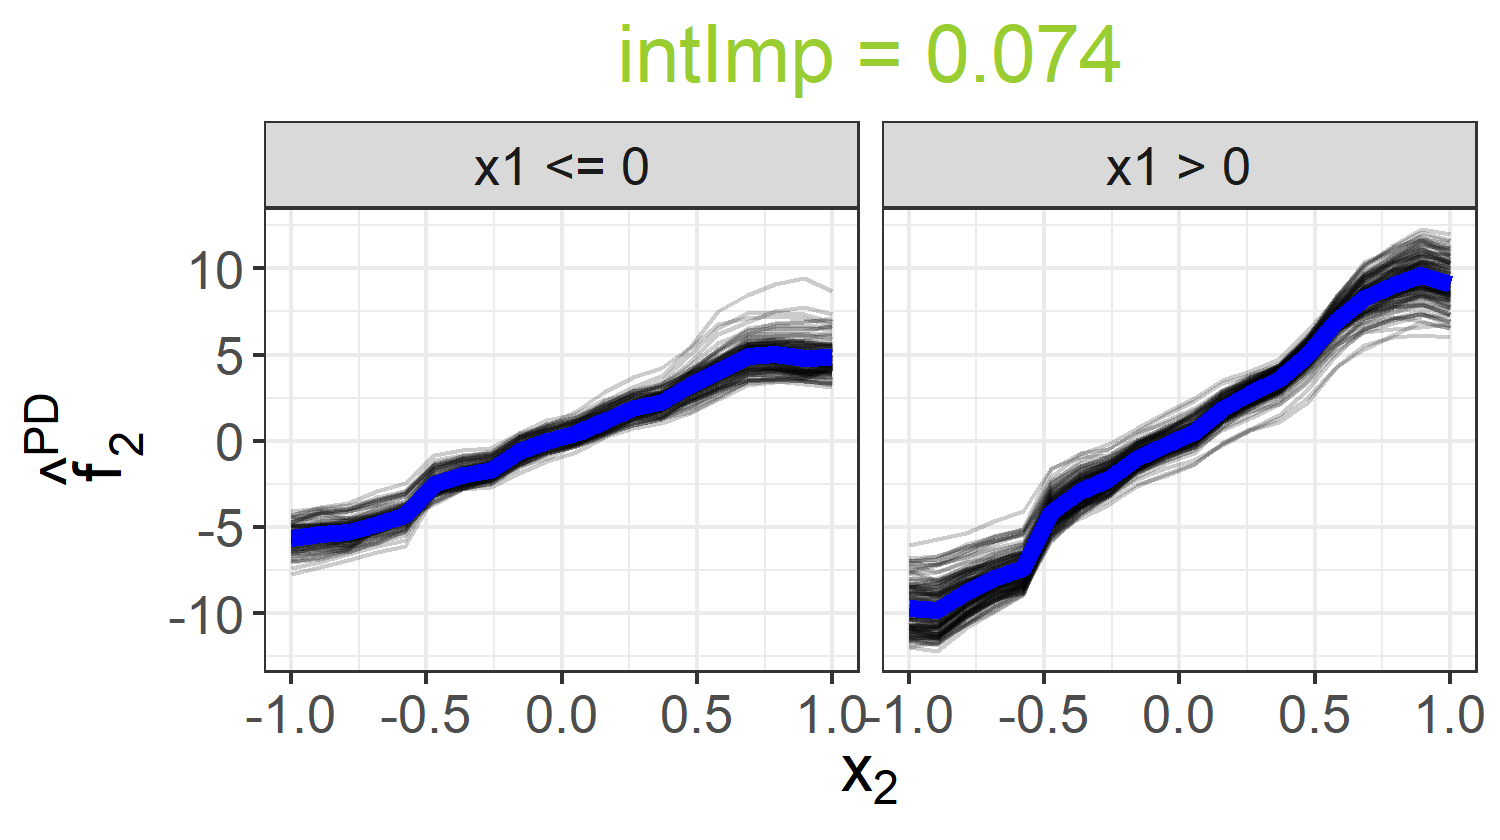
\includegraphics[width=0.37\textwidth]{figure/sim1_dt_split2_1.png}
    % 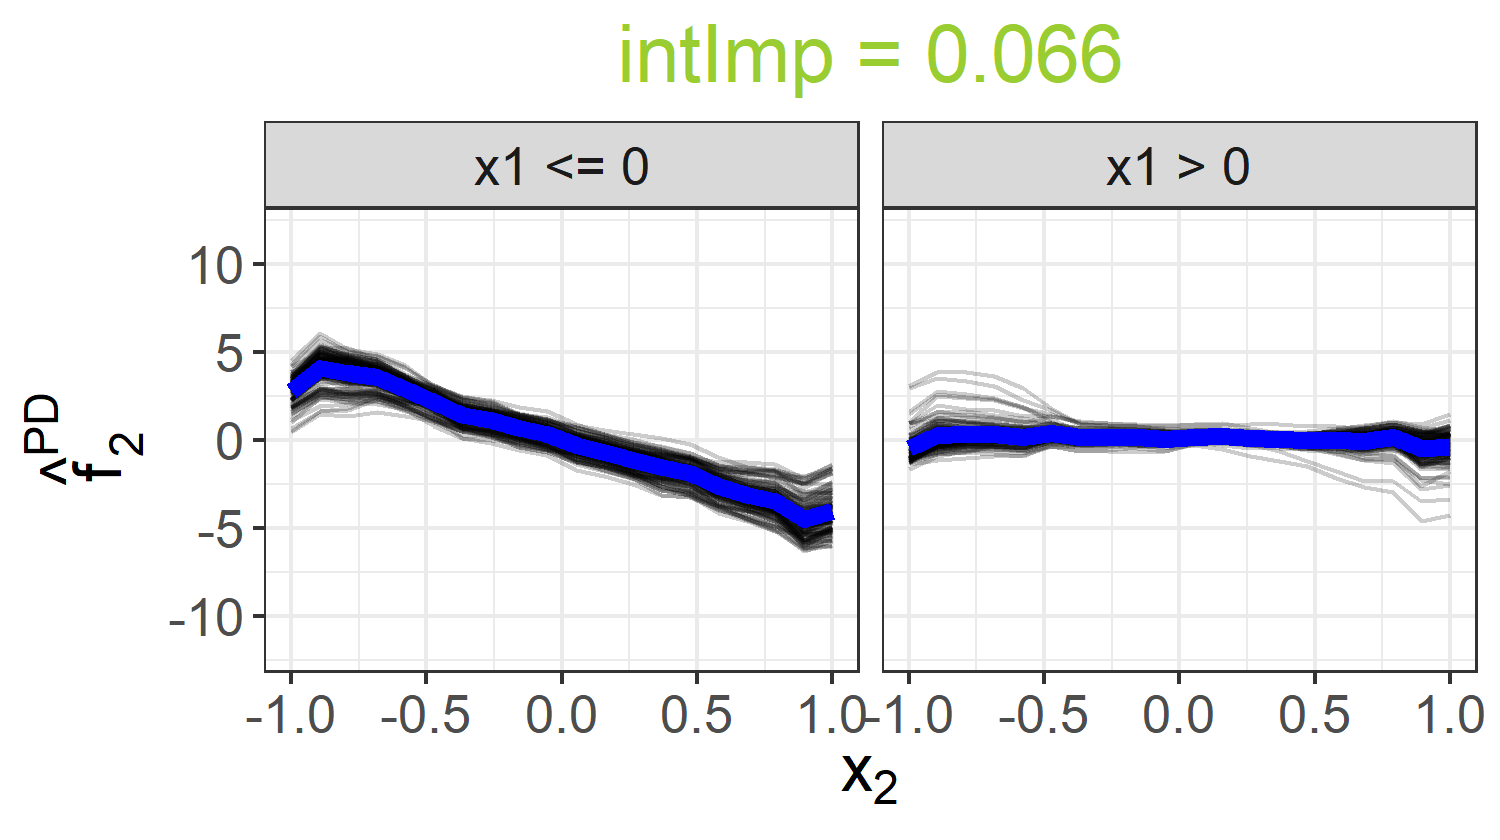
\includegraphics[width=0.37\textwidth]{figure/sim1_dt_split2_2.png}
    
 \vspace{-200px}
    \scriptsize
 \hspace{130px}
 \setlength{\tabcolsep}{1pt}
 \begin{tabular}{|c|c|}
    \hline
       $x_j$ & $intImp_j$  \\\hline
       \rowcolor{ForestGreen!70}
        $\xv_3$     & 0.835 \\
        \rowcolor{YellowGreen!50}
        $\xv_1$     &  0.14\\\hline
    \end{tabular}\\
 \hspace{138px}= 0.975
      %\footnotesize\\
    %\vspace{150px}

    \end{column}

\end{columns}

\end{frame}





\begin{frame}{Outperforming SOTA}

\textbf{Simulation setting}
\begin{itemize}
    \item Draw 1000 i.i.d. samples from $X_1, \ldots , X_4 \sim \mathcal{U}(-1,1)$
    \item True underlying function: $f(\xv) = \sum\nolimits_{j=1}^4 \xv_j + \xv_1 \xv_2 + \xv_2 \xv_3 + \xv_1 \xv_3 + \xv_1 \xv_2 \xv_3 + \epsilon$ % , \epsilon \sim \mathbbm{N}(0, 0.01 \sigma(\mu(\xv))^2)
    \item Fit a correctly specified linear model (interactions with $\xv_4$ are excluded)
    \item 30 repetitions, measure interaction strength between $\xv_2$ and all other 3 features
\end{itemize}

\textbf{Which methods are sensitive to changes in main effect sizes or feature correlations?}


    \begin{table}[thb]
\vspace{.1in}
    \label{tab:simSummary}
    \begin{center}
    \begin{tabular}{|p{5.4cm}|p{1.6cm}|p{1.8cm}|p{1.6cm}|p{1.6cm}|}
    \hline
       Pitfall & REPID & H-Statistic & Greenwell & SHAP  \\\hline
       sensitive to changes of main effect & No & Yes & Yes & No\\\hline
       sensitive to changes of correlation between $\xv_j$ and other features & No & Yes & No & Yes\\
  \hline
    \end{tabular}
    \end{center}
\end{table}
\vspace*{0.2cm}




\end{frame}

\begin{frame}{Outperforming SOTA}
\centerline{
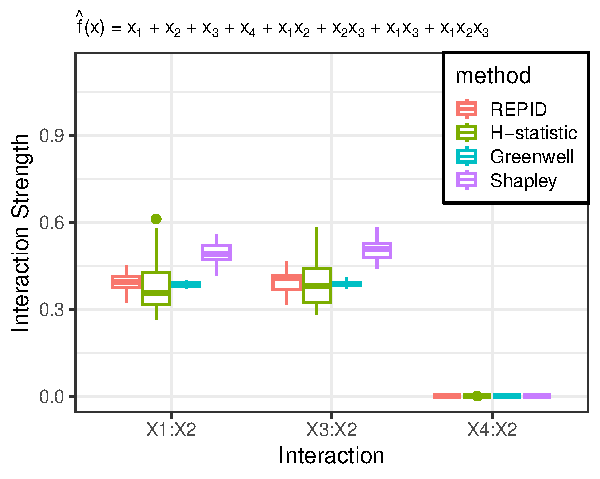
\includegraphics[width=0.4\textwidth, page = 1]{figure/sim_sensi_linear.pdf}
\includegraphics[width=0.4\textwidth, page = 2]{figure/sim_sensi_linear.pdf}
}

   \begin{itemize}
       \item \textbf{Left (initial setting)}: Interaction strength of $\xv_1$:$\xv_2$ and $\xv_3$:$\xv_2$ similar; $\xv_4$:$\xv_2$ no interaction
       \item \textbf{Right}: Set main effect $\beta_1$ = 0.1
       
   \begin{itemize}
       \item \textbf{Expectation}: Interaction strengths should not change
       \item \textbf{Fail}: H-statistic ($\xv_1$:$\xv_2$ > $\xv_3$:$\xv_2$) and Greenwell ($\xv_1$:$\xv_2$ < $\xv_3$:$\xv_2$) 
   \end{itemize}
   \end{itemize}
\end{frame}

\begin{frame}{Outperforming SOTA}
\centerline{
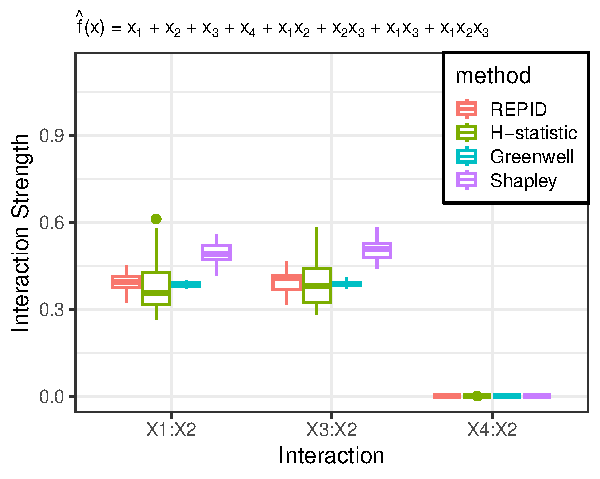
\includegraphics[width=0.4\textwidth, page = 1]{figure/sim_sensi_linear.pdf}
\includegraphics[width=0.4\textwidth, page = 3]{figure/sim_sensi_linear.pdf}
}
  \begin{itemize}
        \item \textbf{Left (initial setting)}: Interaction strength of $\xv_1$:$\xv_2$ and $\xv_3$:$\xv_2$ similar; $\xv_4$:$\xv_2$ no interaction
       \item \textbf{Right}: Increase correlation $\rho(\xv_1, \xv_2) = 0.9$
          \begin{itemize}
       \item \textbf{Expectation}: Interaction strengths should not change
       \item \textbf{Fail}: H-statistic ($\xv_1$:$\xv_2$ < $\xv_3$:$\xv_2$) and Shapley ($\xv_1$:$\xv_2$ > $\xv_3$:$\xv_2$)
   \end{itemize}
       \item[$\rightarrow$] \textbf{REPID is the only method which always leads to correct rankings for these settings}  
   \end{itemize}
   
\end{frame}



\begin{frame}{Limitations of REPID}

\begin{columns}[T, totalwidth = \textwidth]
    \begin{column}{0.48\textwidth}

%\pause
% \textbf{Limitations}:
      \begin{itemize}
  \item[1)] Restricted to one feature of interest \\
  $\Rightarrow$ Different regions for different features \\
  %$\Rightarrow$ No unique decomposition of $\hat{f}(x)$\\%iction function possible\\
  %\item Restricted to ICE curves and PDs $\rightarrow$ not flexible w.r.t. feature effect method
  %\pause
  \item<2->[2)] Restricted to PD (global) and ICE (local) as feature effect methods\\
  $\Rightarrow$ Inherits extrapolation problem\\
  %\phantom{$\Rightarrow$} 
  (unlikely combinations of feature values)
      %\item Feature effect methods based on integrating over marginal distributions such as ICE and PD might extrapolate in unseen or sparse regions (e.g., small $\xv_1$ and high $\xv_3$ values)
      %\item Global/regional effects are not representative w.r.t. the data distribution  
   \item<2->[$\leadsto$] Follow-up GADGET %``Generalized Additive Decomposition of Global feature EffecTs based on interactions'' 
[under review]
  \end{itemize}


        % \begin{itemize}
        %     \item $f(X) = 3X_1\mathbbm{1}_{X_3>0} - 3X_1\mathbbm{1}_{X_3\leq 0} + X_3 + \epsilon$
        %     \item Features uniformly distributed
        %     \item Left: features independent
        %     \item Right: $X_1$ and $X_3$ highly correlated
        %     \item First split: $\xv_3 \leq 0$ (blue) and $\xv_3 > 0$ (orange)
        % \end{itemize}
    \end{column}

    \only<1>{   \begin{column}{0.52\textwidth}
    \centering
    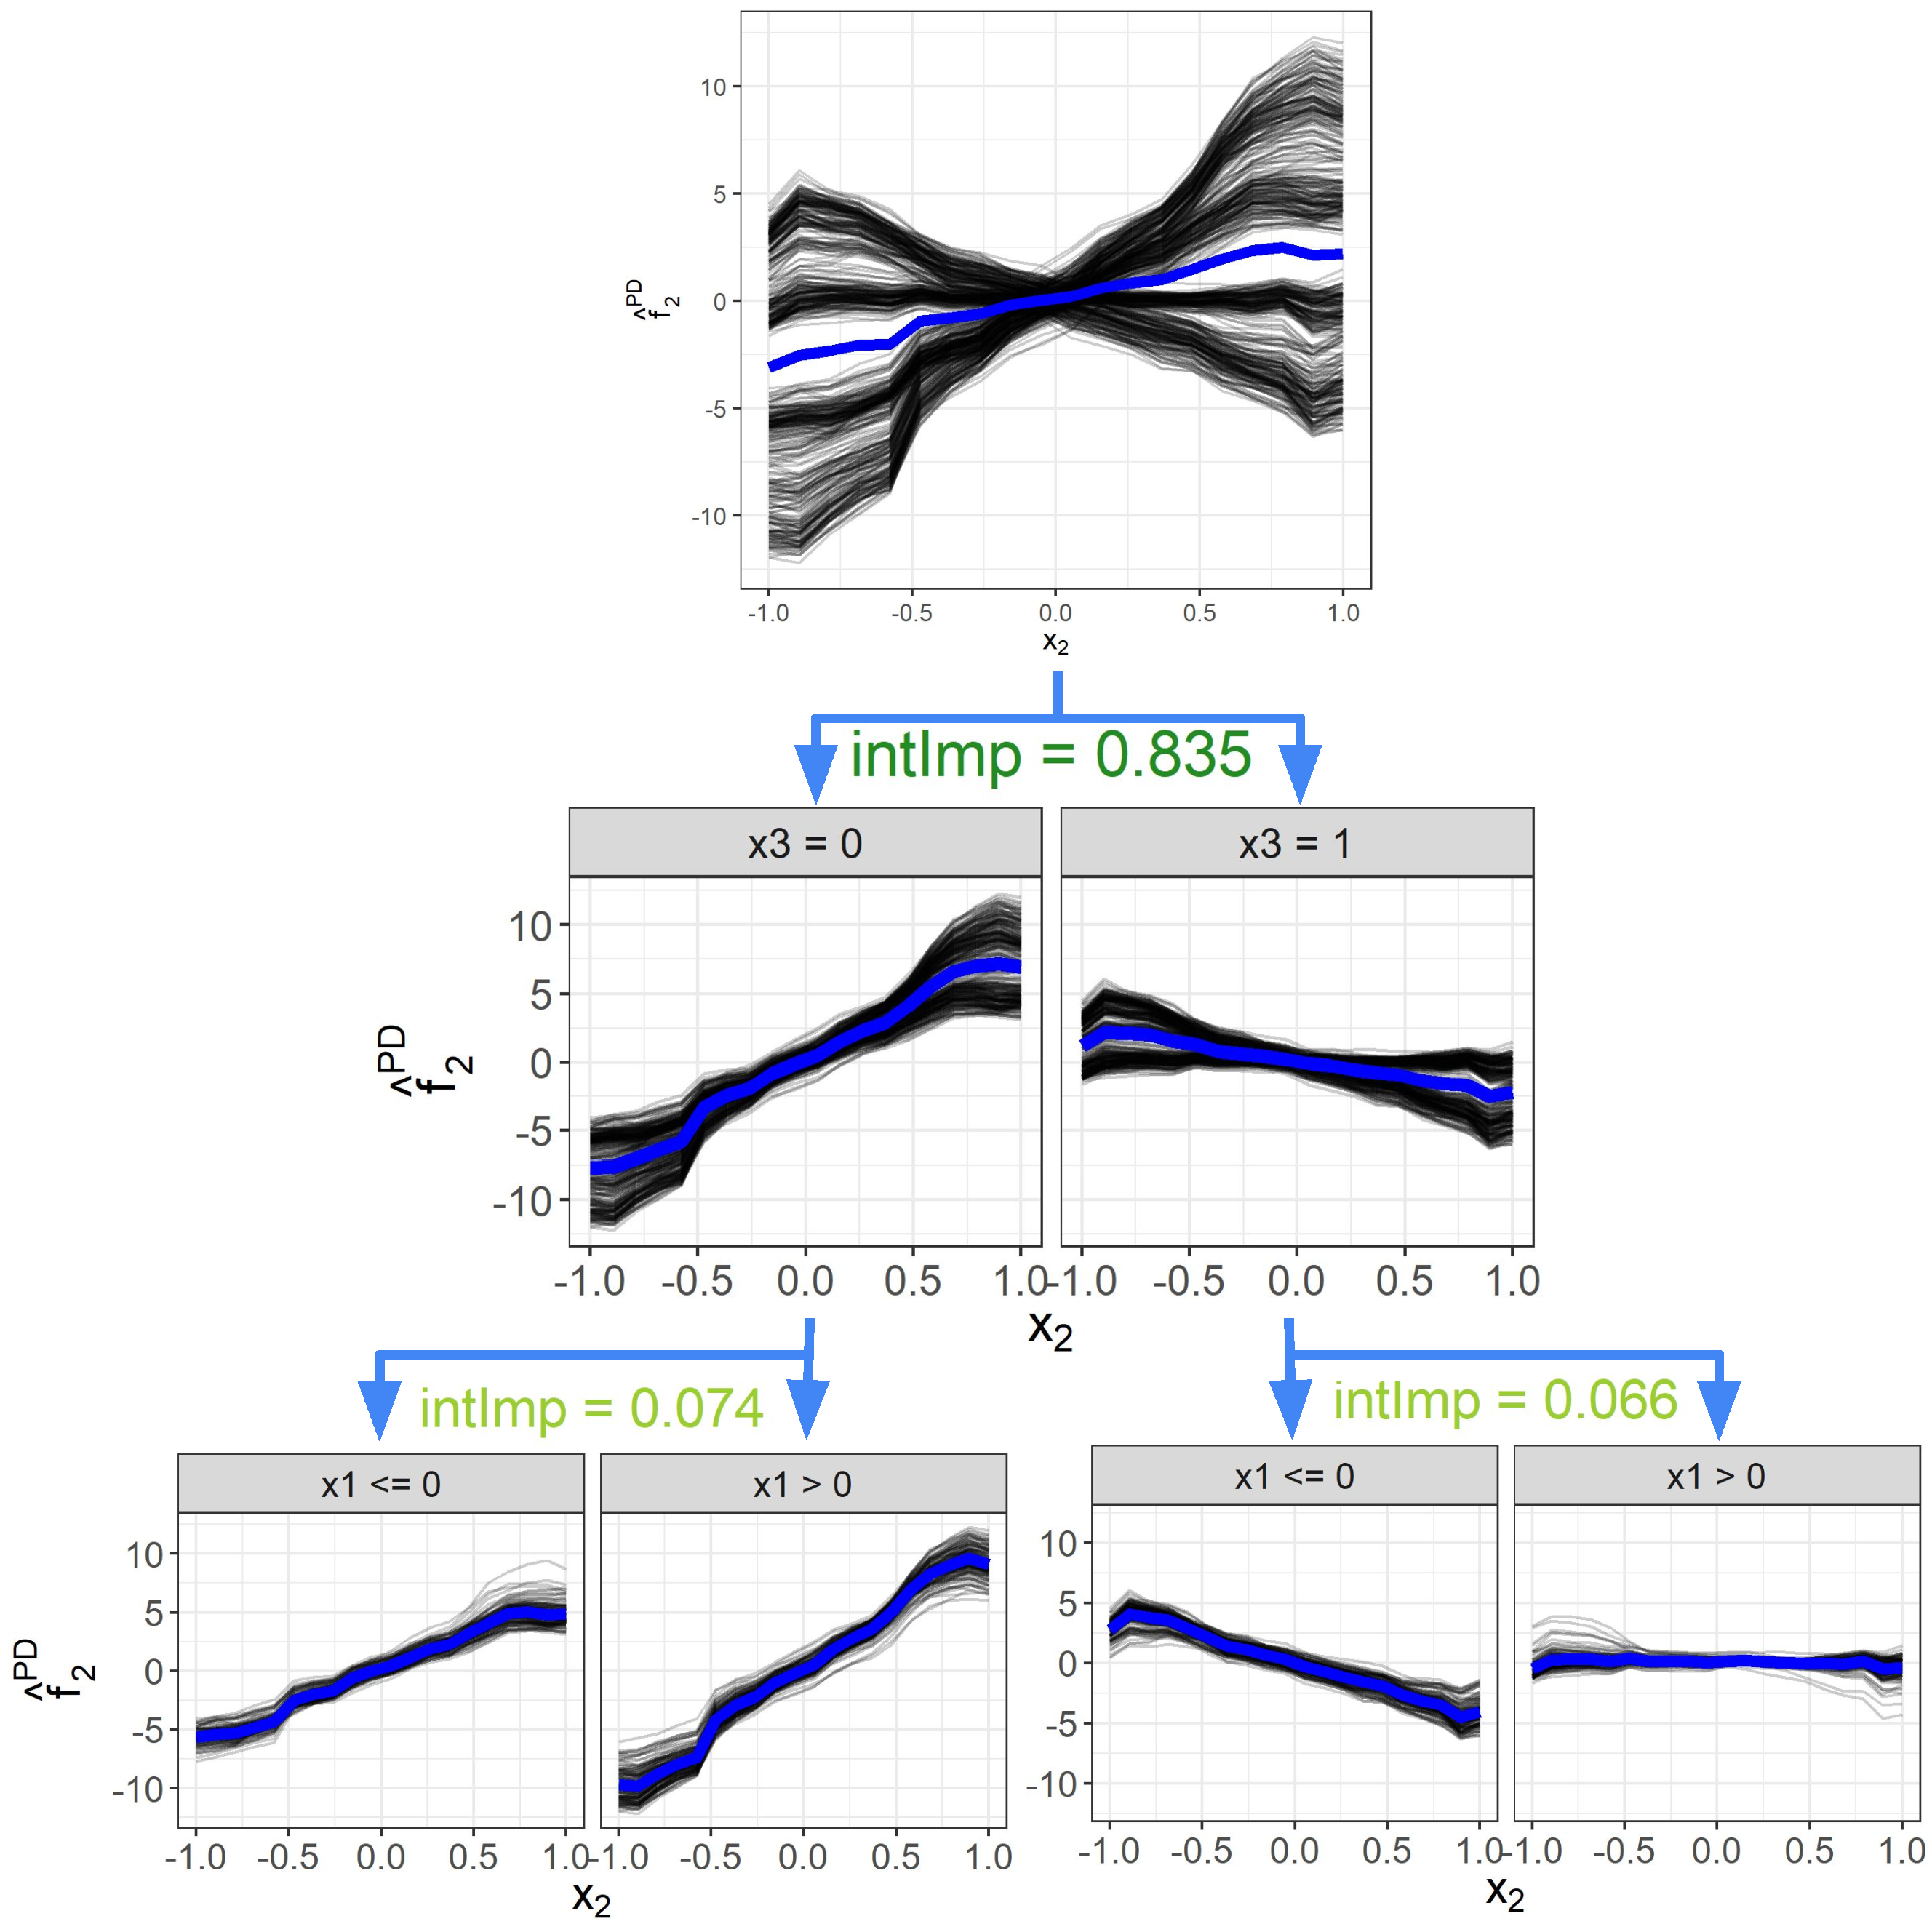
\includegraphics[width=0.95\textwidth]{figure/sim1}
    \vspace{-8pt}
        \begin{columns}[T, totalwidth = \linewidth]
     \footnotesize
            \begin{column}{0.125\linewidth}
            \centering
             $\hat{f}_2^{PD}(X_2)$ %, X_1 > 0 \land X_3 = 0\)\\
         \end{column}
         \begin{column}{0.175\linewidth}
         \centering
             $\approx 8X_2$ %, X_1 > 0 \land X_3 = 0\)\\
         \end{column}
        \begin{column}{0.225\linewidth}
\centering
            $\approx 16X_2$ %, X_1 \leq 0 \land X_3 = 0\)
         \end{column}
        \begin{column}{0.225\linewidth}
        \centering
            $ \approx -8X_2$ %, X_1 \leq 0 \land X_3 \neq 0\)
         \end{column}        
         \begin{column}{0.225\linewidth}
         \centering
             $\approx 0$%, X_1 > 0 \land X_3 \neq 0\)\\
         \end{column}
        \begin{column}{0.025\linewidth}

         \end{column}
     \end{columns}
    \end{column}
}
    \only<2->{\begin{column}{0.52\textwidth}
        %\begin{figure}
      %   \hspace{0.025\linewidth} uncorrelated \hspace{0.225\linewidth} correlated \hspace{0.2\linewidth}
      % \includegraphics[width = \textwidth]{figure/example_repid_extrapol.pdf}
      %      $f(X) = \highlight{3X_1\mathbbm{1}_{X_3>0}} \highlightICE{- 3X_1\mathbbm{1}_{X_3\leq 0}} + X_3 + \epsilon$
      %      \begin{itemize}
      %          \item Left: $X_1, X_2, X_3 \sim \mathbbm{U}(-1,1)$ iid
      %          \item Right: $X_1 = X_3 + \epsilon_1, \epsilon_1 \sim \mathbbm{N}(0, 0.0625)$
      %          \item Model: Tuned feedforward NN
      %          \item Split: $X_3 \leq 0$ (blue), $X_3 > 0$ (orange)
      %      \end{itemize}
      \centering
 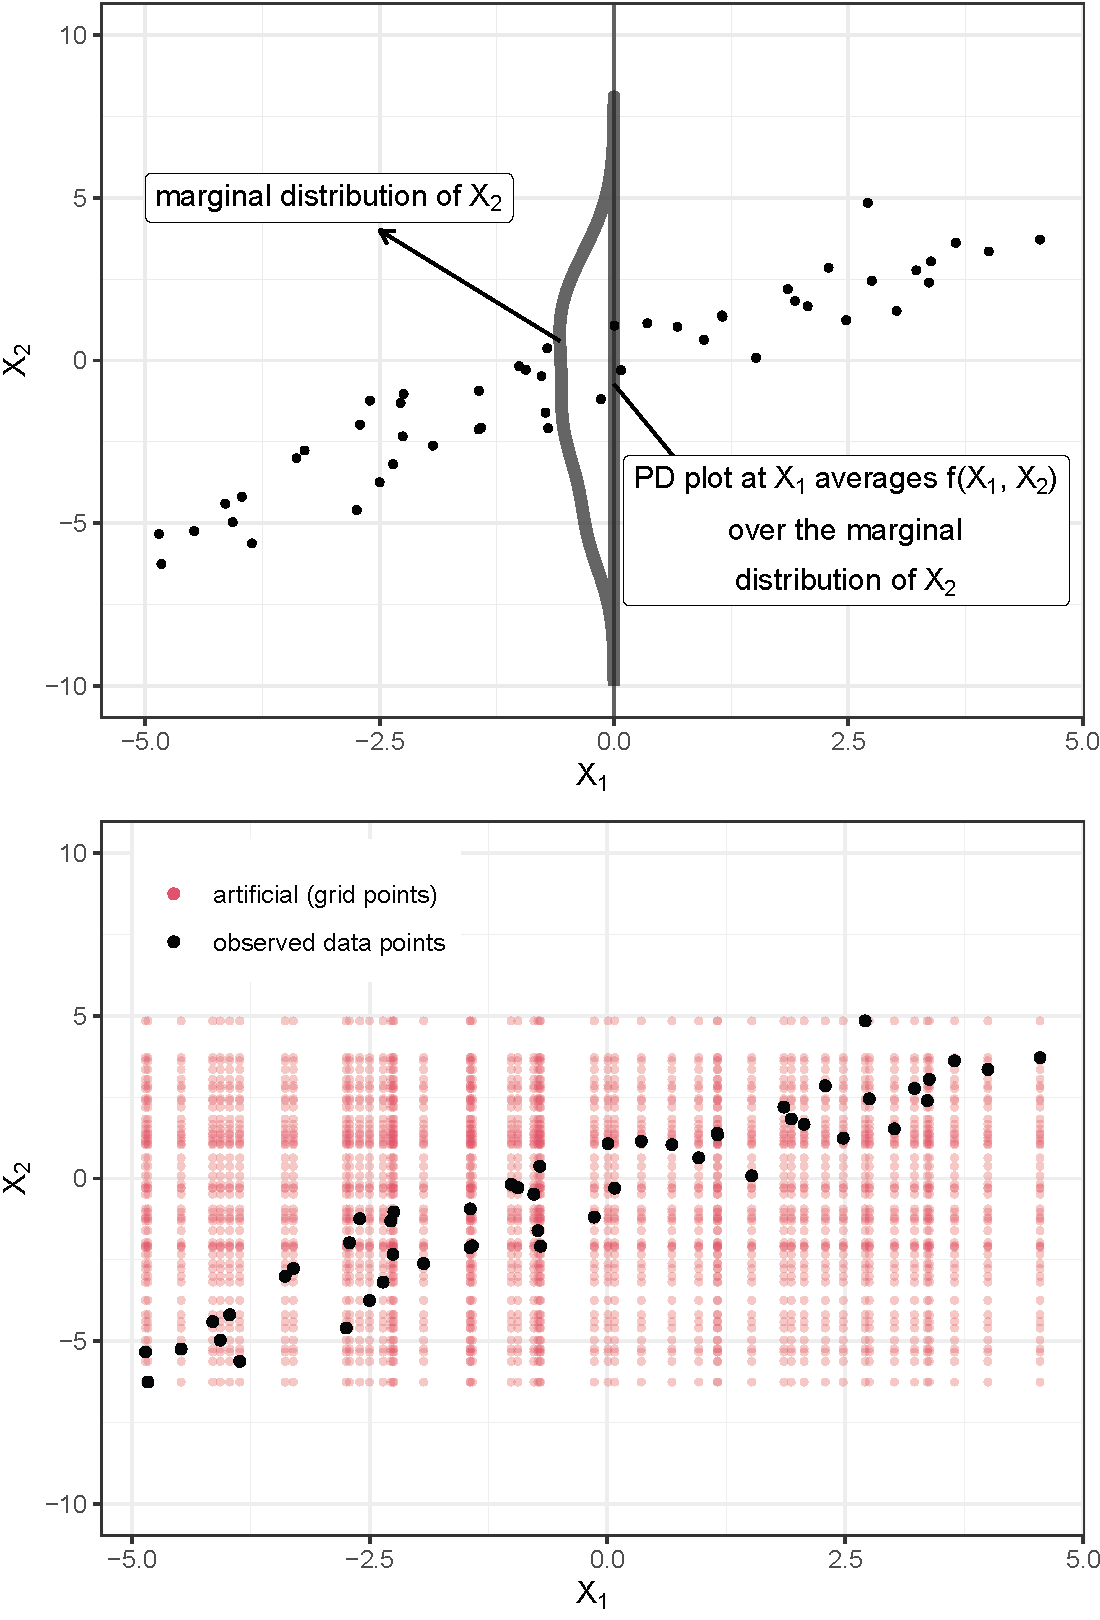
\includegraphics[width = 0.675
 \textwidth]{figure/ale_pdplot.png}
     % \caption{
      %$X_1, X_2, X_3 \sim \mathbbm{U}(-1,1)$ and 
      %$Y = 3X_1\mathbbm{1}_{X_3>0} - 3X_1\mathbbm{1}_{X_3\leq 0} + X_3 + \epsilon$% with $\epsilon \sim \mathbb{N}(0,0.09)$. 
      %left: features independent, right: $X_1$ and $X_3$ highly correlated.
      %$X_1 = X_3 + \delta$ and $\delta \sim \mathbb{N}(0, 0.0625)$. 
      %First split: $\xv_3 \leq 0$ (blue) and $\xv_3 > 0$ (orange).}
  %\end{figure}
    \end{column}}

\end{columns}
\bigskip
\end{frame}


\begin{frame}{Conclusion}

\begin{columns}[T, totalwidth = \textwidth]
    \begin{column}{0.53\textwidth}

 \textbf{Summary of Contributions (REPID)}:
 \begin{itemize}
    \item Regional effects in interpretable regions
    \item Additive decomposition of feature effect 
    %\item Prove meaningfulness of objective - only feature interactions between $\xv_j$ and $\xv_{-j}$ minimized %(measures only feature interactions)
    \item Quantify feature interactions 
    \item Outperforms SOTA interaction indices
    %H-Statistics, Greenwell's and Shapley
\end{itemize}

 \textbf{Summary of Contributions (GADGET)}:
 \begin{itemize}
 \item Unique regions for multiple features
 \item Additive decomposition of prediction function%\\
 \item Extension to ALE and Shapley Dependence
% $\Rightarrow$ TODO: Investigate usefulness as ``approximation'' when terminal regions contain interactions
 \item Test to identify significant interactions
\end{itemize}

        % \begin{itemize}
        %     \item $f(X) = 3X_1\mathbbm{1}_{X_3>0} - 3X_1\mathbbm{1}_{X_3\leq 0} + X_3 + \epsilon$
        %     \item Features uniformly distributed
        %     \item Left: features independent
        %     \item Right: $X_1$ and $X_3$ highly correlated
        %     \item First split: $\xv_3 \leq 0$ (blue) and $\xv_3 > 0$ (orange)
        % \end{itemize}
    \end{column}
    \begin{column}{0.45\textwidth}
    \centering
    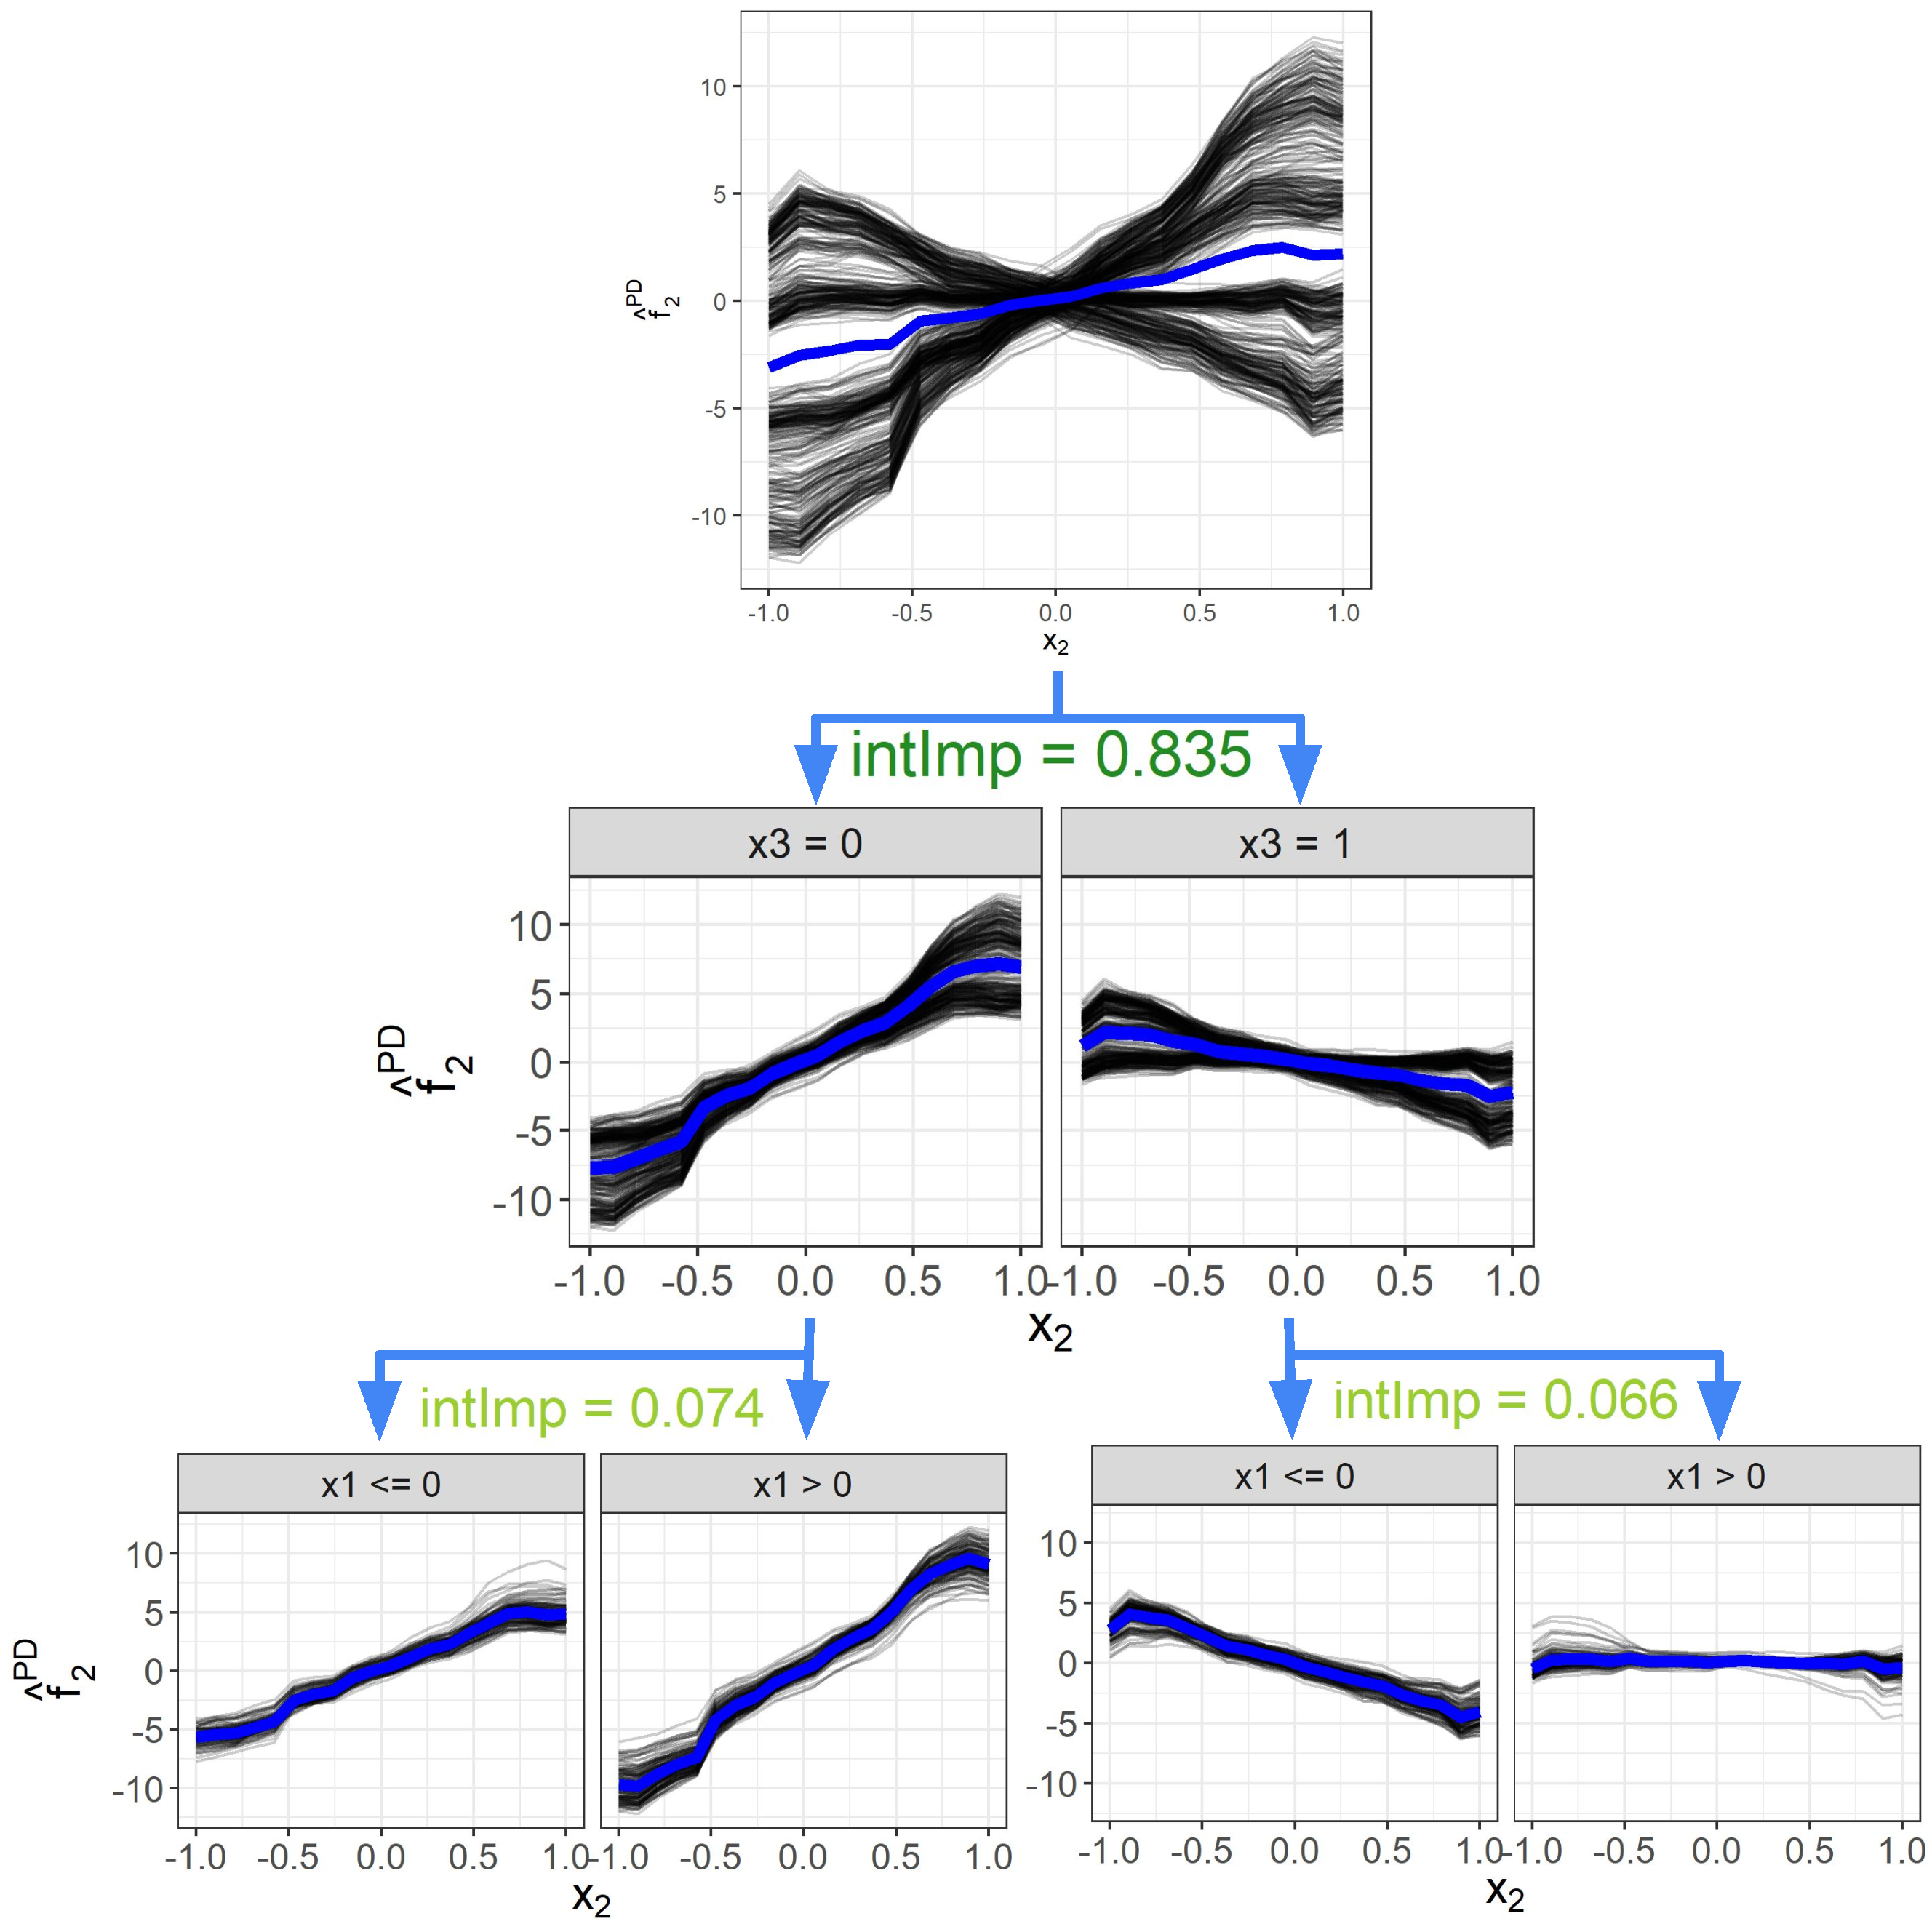
\includegraphics[width=0.95\textwidth]{figure/sim1}
    \vspace{-8pt}
        \begin{columns}[T, totalwidth = \linewidth]
     \footnotesize
            \begin{column}{0.125\linewidth}
            \centering
             $\hat{f}_2^{PD}(X_2)$ %, X_1 > 0 \land X_3 = 0\)\\
         \end{column}
         \begin{column}{0.175\linewidth}
         \centering
             $\approx 8X_2$ %, X_1 > 0 \land X_3 = 0\)\\
         \end{column}
        \begin{column}{0.225\linewidth}
\centering
            $\approx 16X_2$ %, X_1 \leq 0 \land X_3 = 0\)
         \end{column}
        \begin{column}{0.225\linewidth}
        \centering
            $ \approx -8X_2$ %, X_1 \leq 0 \land X_3 \neq 0\)
         \end{column}        
         \begin{column}{0.225\linewidth}
         \centering
             $\approx 0$%, X_1 > 0 \land X_3 \neq 0\)\\
         \end{column}
        \begin{column}{0.025\linewidth}

         \end{column}
     \end{columns}
    \end{column}

\end{columns}

\textbf{Further Directions}: 

Pruning, GADGET as a predictor, comparing regions across models, efficient implementation, more efficient testing and splitting approach, $\dots$
\bigskip
\end{frame}




\endlecture
\end{document}

